% !TEX root =  ../main.tex
\section{Lonely}

\subsection{Definition}

\subsubsection{Signature} \cstr{lonely(s : set<VM>)}

\begin{itemize}
\item \cstr{s} : an non-empty set of VMs for a meaningful constraint. VMs not in the \st{Running} state are ignored.
\end{itemize}

The \cstr{lonely} constraint forces all the running VMs in \cstr{s} to be running on dedicated servers.
Each of the used servers can still host multiple VMs but they have to be in \cstr{s}.

\classification{lonely}{application administrator}{VM placement}{VM-to-VM placement,Partitioning}

\subsubsection{Usage}

The \cstr{lonely} constraint deserves isolation purposes. Hypervisors are supposed
to provide a strong isolation between the VMs. However various attacks, such as those based on 
VM escaping~\cite{wojtczuk},
allow to break this isolation to provide from a malicious VM, a non-legitimate access to the hypervisor or the other VMs.
An application administrator may then want to have to prevent this situation by requiring to have its VMs hosted on servers that do not host unknown, potentially malicious VMs. A \cstr{lonely} constraint can then be used to indicate the VMs that must be running on dedicated servers.

\subsubsection{Example}

Figure~\ref{fig: lonely} depicts a sample reconfiguration between a source and a destination configuration. In this example, the following \cstr{lonely} constraints were considered:

\begin{reconfiguration}
\centering
\begin{minipage}[b]{0.40\textwidth}
\begin{lstlisting}
N1: VM1 VM2
N2: VM3
N3: VM4
N4: VM6
N5: VM5
\end{lstlisting}
\end{minipage}
\begin{minipage}[b]{2cm}
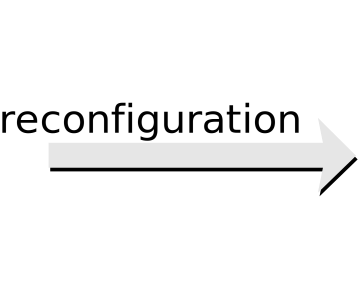
\includegraphics[width=2cm]{img/arrow_reconfiguration}
\end{minipage}
\begin{minipage}[b]{0.40\textwidth}
\begin{lstlisting}
N1: VM1
N2: VM3
N3: VM2 VM4
N4: VM6 VM5
N5:
\end{lstlisting}
\end{minipage}
\caption{A reconfiguration motivated by \cstr{lonely} constraints.}\label{fig: lonely}
\end{reconfiguration}

\begin{itemize}

\item \cstr{lonely(\{VM1,VM3\})}. This constraint was not satisfied in the source configuration as \cstr{VM2}
was colocated with \cstr{VM1} despite \cstr{VM2} does not belong to the VMs given as parameter.
This violation was fixed by relocating \cstr{VM2} to \cstr{N3}.

\item \cstr{lonely(\{VM2, VM4\})}. This constraint was not satisfied in the source configuration. It was fixed by
colocating \cstr{VM2} with \cstr{VM4} on \cstr{N3}.

\item \cstr{lonely(\{VM5, VM6\})}. This constraint was satisfied in the source configuration.
The constraint is still satisfied in the destination configuration despite the relocation of \cstr{VM5} to
\cstr{N4} which is allowed by the constraint.
\end{itemize}


\fullVersion{
\subsection{Model}

This constraint is modeled using a restriction on the demanding slice associated to each of the running VMs.

\begin{equation*}
\begin{split}
\forall V \subseteq \mathcal{V}, \ lonely(V) \triangleq&\\
   & \forall v_i,v_j \in V, d_i^h =  d_j^h
\end{split}
\end{equation*}

\subsection{Violation Detection}

The detection of the violating elements in \cstr{lonely} consists in computing every VMs that are not
in the given set of VMs, but running on servers hosting the given VMs.


\subsection{Availability}

\subsubsection{In {\btrp}}

This constraint is available in {\btrp} since the version 2.1 using the name \texttt{Lonely}. 
Two groups of placement variables are created. One containing the placement variables of the given VMs, the other containing the other VMs running on the servers. One \emph{disjoint} ensures then
no variables in different groups, are instantiated to the same value.

\begin{equation*}
\begin{split}
\forall V \subseteq \mathcal{V}, \ lonely(V) \triangleq&\\
   & \forall v_i,v_j \in V, eq(d_i^h, d_j^h)
\end{split}
\end{equation*}

\subsubsection{In Amazon EC2}

The constraint is available on Amazon EC2 under the terms of \emph{dedicated instances}~\cite{amazon-lonely}.
}

\subsection{See also}

%\subsubsection{Context relative constraints}

%\begin{itemize}
%\item \cstrref{split}: The \cstr{split} constraint is a generalization of the \cstr{lonely} constraint. It states that the two set of VMs, given as arguments,  must not share servers. A \cstr{lonely} constraint can then be emulated using a \cstr{split} constraint when the second set of VMs is the absolution complement of the first one.
%\end{itemize}

%\subsubsection{Emulating the \cstr{lonely} constraint}
\emulatedWith{lonely}{split}{\cstr{lonely(vs1)}}{\cstr{split(\{vs1,\oline{vs1}\})}}
\printListOfInheritance{lonely}
%\begin{itemize}
%\item 
%\end{itemize}
%
%\subsubsection{Available specializations of the \cstr{lonely} constraint}




